\documentclass[12pt,a4paper]{article}
\usepackage{composites2019}

\begin{document}
\thispagestyle{empty}

\vspace*{-3.4cm}
\begin{table}[!h]
\begin{tabular}{r}
\hspace*{2.9cm} \scriptsize \textsf{7th ECCOMAS Thematic Conference on the Mechanical Response of Composites: COMPOSITES 2019} \\
\hspace*{2.9cm} \tiny \textsf{A. Turon, P. Maimí \& M. Fagerström (Editors)}
\end{tabular}
\end{table}

\vspace*{-0.7cm}

\begin{center}
\title{INSTRUCTIONS TO PREPARE A ONE PAGE ABSTRACT FOR THE ECCOMAS CONFERENCE: COMPOSITES 2019}
\end{center}
\begin{center}
\textbf{\underline{Luca Di Stasio}$^{1,2,*}$, Janis Varna$^{2}$, Zoubir Ayadi$^{1}$} \\ [7pt]
\small{$^1$~Affiliation number one}  \\  [2pt]
\small{$^2$~Affiliation number two}  \\  [2pt]
\small{$^*$~\texttt{luca.di.stasio@ltu.se}} \\
\end{center}

\noindent
The abstracts accepted for the conference will be published in the Book of Abstracts. The abstracts should briefly outline the main features, results and conclusions of the research, as well as their general significance. The abstract is one page long and has to be written in English with a Times New Roman 12 points single spaced font. Figures and tables should may be included with captions, see Figure \ref{fig:Claustre}. The figures and tables should be referred to in the text. The title should be written with all capital letters. The abstract must contain the full names and affiliations of all the authors and the e-mail address of the corresponding author. His/her name is to be underlined in the author list. References can be added as well~\cite{Barbero,Pimenta}.

\begin{figure}[h]
\centering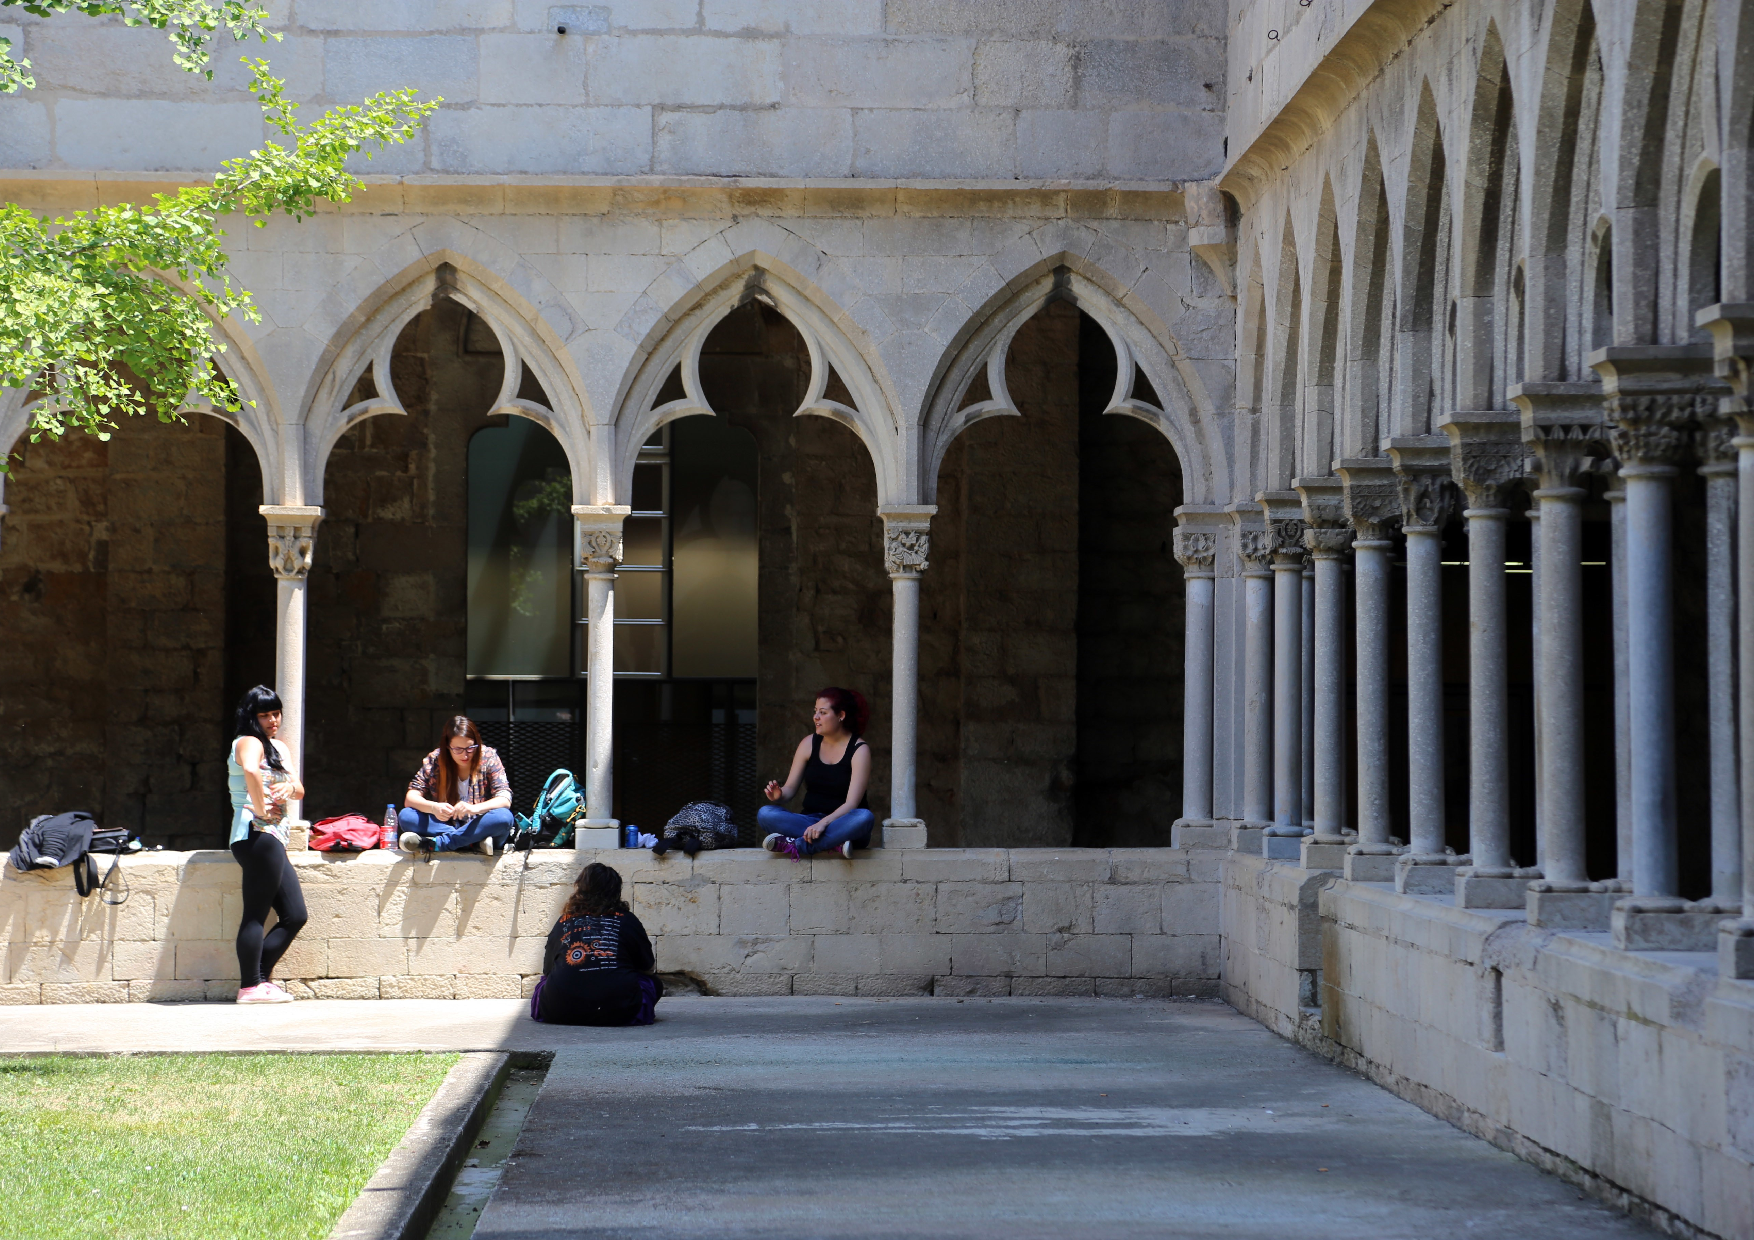
\includegraphics[width=0.55\linewidth]{Claustre.pdf}
\caption{The former cloister of the convent of St. Domènec, which is the venue of this conference.}
\label{fig:Claustre}
\end{figure}


Authors should upload the abstract via the website \texttt{composites2019.udg.edu} no later than \textbf{January 17, 2019}. 

\begin{thebibliography}{9}

% === Replace this by your references ===

\bibitem{Barbero} E.J. Barbero (2008) \textit{Finite Element Analysis of Composite Materials}. CRC Press, Boca Raton.
\bibitem{Pimenta} S. Pimenta and S.T. Pinho (2012) The effect of recycling on the mechanical response of carbon fibres and their composites. \textit{Composite Structures}, \textbf{94}, 3669-3684.

\end{thebibliography}
\end{document}
  
